\documentclass[a4paper,11pt,oneside,openany]{jsbook}
%
\usepackage{amsmath, amssymb}
\usepackage{bm}
\usepackage[dvips,dvipdfmx]{graphicx}
\usepackage{verbatim}
\usepackage{wrapfig}
\usepackage{ascmac}
\usepackage{makeidx}
\usepackage{enumerate}
\usepackage{comment}
\usepackage{multirow}
\usepackage{listings}

\usepackage[hang,small,bf]{caption}
\usepackage[subrefformat=parens]{subcaption}
\captionsetup{compatibility=false}

%%% 余白・文字数調整(左37mm, 右18mm, 上下共30mm, 文字数約40字/行, 行数約32行)
\setlength{\textwidth}{160truemm}      % テキスト幅: 210-(37+18)=155mm
\setlength{\fullwidth}{\textwidth}     % ページ全体の幅
\setlength{\oddsidemargin}{25truemm}   % 左余白
\addtolength{\oddsidemargin}{-1truein} % 左位置デフォルトから-1inch
\setlength{\topmargin}{20truemm}       % 上余白
\setlength{\textheight}{247truemm}     % テキスト高さ: 297-(30+30)=237mm
\addtolength{\topmargin}{-1truein}     % 上位置デフォルトから-1inch
\makeatother
%
\def\linesparpage#1{\baselineskip=\textheight
   \divide\baselineskip by #1}
\def\kcharparline#1{%
   \ifx\xkanjiskip\undefined%
   \jintercharskip 0mm plus 0.2mm minus 0.2mm
   \else
   \xkanjiskip 0mm plus 0.2mm minus 0.2mm
   \fi
   \settowidth{\textwidth}{}%
   \multiply\textwidth by #1}
%
\newcommand\figref[1]{\textbf{図~\ref{fig:#1}}}
\newcommand\tabref[1]{\textbf{表~\ref{tab:#1}}}
\newcommand{\bhline}[1]{\noalign{\hrule height #1}}

\begin{document}

% \begin{titlepage}

% \begin{center}
% {\Large 令和3年度 卒業論文}\\ % タイトル
% \vspace*{150truept}
% {\huge 評価者特性の時間変動を考慮した\\項目反応モデル}\\ % タイトル
% \vspace{120truept}

% {\huge 電気通信大学 情報理工学域I類}\\ % 所属
% \vspace{10truept}
% {\huge コンピュータサイエンスプログラム}\\ % 所属
% \vspace{10truept}
% {\huge 学籍番号 1810519}\\ % 学籍番号
% \vspace{50truept}
% {\huge 林 真由}\\ % 著者
% \vspace{50truept}
% {\huge 指導教員:宇都雅輝 准教授}\\
% \vspace{50truept}
% {\huge 2022年1月31日}\\ % 提出日
% \end{center}
% \end{titlepage}
% \kcharparline{40} % 一行を40字に

% \frontmatter
% %%% 論文要旨
% \addcontentsline{toc}{chapter}{論文要旨}
% 近年,大学入試や資格試験,教育評価などの場において,パフォーマンス評価は重要な役割を果たしている.一方で,パフォーマンス評価では,評価者の厳しさや一貫性の違い,各得点の使用傾向の差などにより,採点に偏りが生じ,受検者の能力を正確に測ることが難しいという問題がある.この問題を解決するために,評価者特性の影響を考慮して受検者の能力を推定できる項目反応モデルが多数提案されている.
% これらのモデルは評価者の基準が採点過程で変化しないという仮定のもと成り立っているが,多数の受験者を長時間かけて採点するような場合には,この仮定は成り立たないことがある.このような評価者の採点基準が採点過程で変化する特性は評価者ドリフト(Rater Drift)と呼ばれ,これを考慮したモデルについても提案がなされている.既存モデルでは,評価者の厳しさの初期値と傾きを表すパラメータを導入することで,評価者特性の時間変化を捉えるモデルとなっているが,このモデルでは,評価者特性の変化を直線的にしかとらえることができない.この問題を解決するために,本研究では,時間区分ごとの評価者の厳しさを推定する新しい項目反応モデルを提案する.また,シミュレーション実験と実データ実験を通して提案モデルの有効性を示す.
\tableofcontents
%
%
\mainmatter

\newpage
\chapter{はじめに}
近年,受検者の論理的思考力や表現力などの実践的な能力を測定する方法の一つとして,パフォーマンス評価が注目されている.大学入学共通テストでも,論述式問題を採用する議論がなされていた.他方で,パフォーマンス評価における問題の一つが,採点の信頼性に関わる点である.パフォーマンス評価では,評価者の厳しさや一貫性の違い,各得点の使用傾向の差などにより,採点に偏りが出てしまうことがあり,このことが評価の信頼性低下の要因となる.このような問題は大学入試や資格試験,教育評価などにおける,レポート課題,グループディスカッションやプレゼンテーション課題などの様々なパフォーマンス評価場面で起こり得る.この問題を解決するために項目反応理論(Item response theory:IRT)\cite{IRTtext,IRTLord}と呼ばれる数理モデルの利用が近年注目されている.IRTは,コンピュータ・テスティングの普及とともに,近年様々な分野で実用化が進められている数理モデルを用いたテスト理論の一つで,テストを作成・実施・評価・運用するための数理モデルである.

一般的な客観式テストに適用されるIRTモデルは,受検者の能力と課題の困難度の2つのパラメータからなるモデル\cite{rash}である.しかし,それらのモデルは複数の評価者が採点を行うパフォーマンス評価には適用することができない.なぜなら,評価者によって一貫性や厳しさは様々であるが,従来のモデルではそのような特性差を考慮できないためである.この問題を解決するために,評価者特性を表すパラメータを加えたIRTモデルが近年多数提案されている\cite{raterRash,rater2,rater3,Patz}.これらのモデルは,受検者の能力と課題の困難度の他に,評価者の厳しさや一貫性の違い,各得点の使用傾向の差などをパラメータとして加えたモデルであり,これを利用することで評価者の特性差の影響を考慮した受検者の能力推定が可能となる.

これらのモデルは評価者の基準が採点過程で変化しないという仮定のもと成り立っている.しかし,多数の受検者を長時間かけて採点するような場合,評価者の特性が採点の過程で変化する評価者ドリフト(Rater Drift)と呼ばれる現象がしばしば生じる.評価者ドリフトが生じている場合に,評価者の基準が変化しないと仮定したモデルを適用してしまうと,適切な評価者特性の推定を行うことができず,能力推定値にもバイアスが生じると考えられる.
この問題を解決するために,評価者特性の時間変動を考慮したIRTモデルが提案されている\cite{raterdrift}.このモデルは,評価者が行なった一連の評価を時間区分で区切り,評価者の初期の厳しさと厳しさの傾きを使用して評価者特性の時間変化を捉えるモデルとなっている.
しかし,既存モデルの問題点として次の点が挙げられる.
\begin{enumerate}
  \item 評価者特性の変化を直線的にしかとらえることができない
  \item 評価者の一貫性と各得点に対する基準の差異を考慮できていない.
\end{enumerate}  

以上の問題を解決するため,時間区分ごとの評価者の厳しさを推定できる新しいIRTモデルを提案する.具体的には,各時間区分における評価者の厳しさパラメータを導入し,そのパラメータにマルコフ性を仮定して推定するモデルを提案する.また,提案モデルには,評価者の一貫性と,各段階得点に対する各評価者の基準の差異を考慮したパラメータも付与する.提案モデルの利点は次のとおりである.
\begin{enumerate}
  \item 時間区分ごとの評価者特性の変化をより柔軟に推定することができるため,データへのモデル適合度が向上し,モデルの性能が改善する.
  \item 評価者ごとの一貫性の差異,及び各段階得点に対する基準の差異をより柔軟に考慮できるため,データへのモデル適合度が向上し,モデルの性能が改善する.
\end{enumerate}
本研究では,シミュレーション実験および実データ実験を通して提案モデルの有効性を示す.
\newpage

\chapter{項目反応理論}
本研究は,課題・評価者・時間区分の特性を考慮した高精度な能力推定を行うことを目的とする.このような能力推定を実現するために,本研究ではIRTを利用する.

IRTは,コンピュータ・テスティングの普及とともに,近年様々な分野で実用化が進められている数理モデルを用いたテスト理論の一つで,テストを作成・実施・評価・運用するための実践的な数理モデルである\cite{IRTtext,IRTLord}.IRTの利点として,次のような点が挙げられる\cite{IRTUtoUeno}.
\begin{itemize}
\item 推定制度の低い異質項目の影響を小さくして能力推定を行うことができる.
\item 異なる項目への受検者の反応を同一尺度上で評価できる.
\item 欠測データから容易にパラメータを推定できる.
\end{itemize}

IRTはこれまで,正誤判定問題や選択式問題などの正誤を一意に判定できる2値型データを扱うテストへの利用が一般的であった. 一方で,近年では論述式・記述式試験のような多段階カテゴリを用いた評価データに対して,多値型IRTモデルを適用してパフォーマンスを評価する応用的な研究も進められている\cite{IRTMatteucci,IRTDeCarlo}.
次節では,IRTにおける基礎的なモデルとして,2値型データを扱うモデルについて述べる.その後,その拡張であり,本研究で扱うリッカート型データに適用できる代表的な多値型IRTモデルを紹介する.

\section{2値型項目反応モデル}
最も基礎的なIRTモデルとしては,ラッシュモデル\cite{rash}が知られている.ラッシュモデルでは,受検者$j$が項目$i$に正答する確率を次の式で表す.

\begin{equation}
P_{ij} = \frac{\mathrm{exp}(\theta_{j}-b_{i})}{1 + \mathrm{exp}(\theta_{j}-b_{i})}
\end{equation}

ここで,$\theta_{j}$は受検者$j$の能力,$b_{i}$は項目$i$の困難度を表す.

ラッシュモデルは,少数のパラメータで表現されているため,少数データからでも高精度にパラメータを推定できる\cite{rashbenefit}.しかし,そのモデルの単純さにより,複雑な特性を表現できないため,データへの当てはまりが悪い場合が多い\cite{rashloss}.
そのため,実際には,ラッシュモデルに項目$i$の識別力パラメータ$\alpha_{i}$を加えた2母数ロジスティックモデルを使用することが一般的である.2母数ロジスティックモデルでは,受検者$j$が項目$i$に正答する確率を次の式で表す.

\begin{equation}
  P_{ij} = \frac{\mathrm{exp}(\alpha_{i}(\theta_{j}-b_{i}))}{1 + \mathrm{exp}(\alpha_{i}(\theta_{j}-b_{i}))}
  \end{equation}
  
ここで,$\alpha_{i}$は項目$i$の識別力を表す.識別力$\alpha_{i}$の値が大きいほど,能力値$\theta = b_i$付近の能力を高い精度で識別できる.

ラッシュモデルや2母数ロジスティックモデルは, テスト項目に対する受検者の反応が,正誤のような2値データで表される場合に適用できる.しかし,本研究のようなパフォーマンス評価では,段階的な評価カテゴリ(得点)が対応づけられた評価基準に基づいて採点を行うことが多いため,評価データは多値データとなることが一般的である.このような多値データに適用できるモデルとして,2値型IRTモデルを拡張した多値型IRTモデルが提案されてきた.


\section{部分採点モデル(PCM)}
Mastersによって提案された多値型IRTモデルとして,部分採点モデル(Partial Credit Model)\cite{PCM}が知られている.PCMでは, 受検者$j$が項目$i$に対してカテゴリ$k \in \{1\dots K\}$と反応する確率$P_{ijk}$を次の式で表す.
\begin{equation}
P_{ijk} = \frac{\mathrm{exp}\sum_{m=1}^{k}(\theta_{j}-\beta_{im})}{\sum_{l=1}^{k} \mathrm{exp}\sum_{m=1}^{l}(\theta_{j}-\beta_{im})}
\end{equation}
ここで,$\beta_{ik}$は項目$i$においてカテゴリ$k-1$からカテゴリ$k$に遷移する困難度を表し,ステップパラメータと呼ばれる.PCMではモデル識別性のために$\beta_{i0}=0$を所与とする.

PCMでは,カテゴリ$k$への反応確率$P_{ijk}$とカテゴリ$k-1$への反応確率$P_{ijk-1}$のロジットlog($P_{ijk}/P_{ijk-1}$)を受検者の能力とカテゴリ$k$における項目困難度の線形和$\theta_{j}-\beta_{ik}$で定義しており,項目への正答確率と誤答確率のロジットを$\theta_{j}-\beta_{i}$と定義するラッシュモデルの多値への一般化と解釈できる.

\section{一般化部分採点モデル(GPCM)}
Murakiは,PCMにおける項目識別力一定の制約を緩和したモデルとして,一般化部分採点モデル(Generalized Partial Credit Model:GPCM)\cite{GPCM}を提案している.GPCMでは受検者$j$が項目$i$に対してカテゴリ$k$と反応する確率$P_{ijk}$を次の式で表す.
\begin{equation}
P_{ijk} = \frac{\mathrm{exp}\sum_{m=1}^{k}(\alpha_{i}(\theta_{j}-\beta_{im}))}{\sum_{l=1}^{K} \mathrm{exp}\sum_{m=1}^{l}(\alpha_{i}(\theta_{j}-\beta_{im})}
\end{equation}
PCMと同様に,モデル識別性のため,$\beta_{i0}=0$を所与とする.

GPCMは,Andrichによる評定尺度モデル\cite{RSM}と同様に,ステップパラメータ$\beta_{ik}$を$\beta_{i}+d_{k}$,あるいは$\beta_{i}+d_{ik}$と分解することができ,以下のようなモデルで表されることもある.
\begin{equation}
P_{ijk} = \frac{\mathrm{exp}\sum_{m=1}^{k}(\alpha_{i}(\theta_{j}-\beta_{i}-d_{im}))}{\sum_{l=1}^{K} \mathrm{exp}\sum_{m=1}^{l}(\alpha_{i}(\theta_{j}-\beta_{i}-d_{im})}
\end{equation}
\begin{equation}
P_{ijk} = \frac{\mathrm{exp}\sum_{m=1}^{k}(\alpha_{i}(\theta_{j}-\beta_{i}-d_{m}))}{\sum_{l=1}^{K} \mathrm{exp}\sum_{m=1}^{l}(\alpha_{i}(\theta_{j}-\beta_{i}-d_{m})}
\end{equation}
ここで,$\beta_{i}$は項目$i$の困難度パラメータ,$d_{ik}$は項目$i$のカテゴリ$k$に対する閾値パラメータ,$d_k$はカテゴリ$k$のカテゴリパラメータと呼ばれる.モデルの識別性のために,$d_{i1}=0,\sum_{k=2}^{K}d_{ik}=0,d_1=0,\sum_{k=2}^{K}d_{k}=0$を所与とする.

\newpage

\chapter{評価者特性を考慮した項目反応モデル}
これまで紹介してきたIRTモデルは,受検者とテスト項目の2相データへの適用を想定している.一方で,本論で想定するパフォーマンス評価データ$X$は,パフォーマンス課題$i\in \{1\dots I\}$に対する受検者$j\in \{1\dots J\}$のパフォーマンスに評価者$r\in \{1\dots R\}$が与える評点$k\in \{1\dots K\}$の集合であり,以下のような3相データとして定義される.
\begin{equation}
X = \{x_{ijr}\arrowvert x_{ijr} \in \{-1,1,\dots, K\}\}(i\in \{1\dots I\},j\in \{1\dots J\},r\in \{1\dots R\})
\end{equation}
このような3相データに対して,これまで紹介した一般的なIRTモデルを直接適用することはできない.この問題の解決策として,評価者特性を表すパラメータを加えたIRTモデルが提案されてきた(e.g.,\cite{raterRash,rater2,rater3}).これらのIRTモデルは,従来のIRTモデルにおいて,項目パラメータを課題の特性を表すパラメータとみなし,評価者特性を表すパラメータを付与したモデルとして定式化される.
\section{多相ラッシュモデル}
多相データのためのIRTモデルとして,最も広く知られているモデルは,Linacreが提案した多相ラッシュモデル(MFRM: many-facet Rasch
model)\cite{raterRash}である.MFRMは,ラッシュモデルに,課題と受検者以外の要因を表すパラメータを付与したモデルである.例えば,評価者$r$の評価の厳しさを表すパラメータ$\beta_{r}$を付与した多相ラッシュモデルでは,評価者$r$が課題$i$における受検者$j$のパフォーマンスにポジティブな判定を与える確率を次式で与える.
\begin{equation}
P_{ijr}=\frac{\mathrm{exp}(\theta_{j}-b_{i}-\beta_{r})}{1+\mathrm{exp}(\theta_{j}-b_{i}-\beta_{r})}
\end{equation}
ここで,$b_i$は課題$i$の困難度を表す.
MFRMは2値データを扱うモデルであるが,ラッシュモデルと同様に,PCMを用いた多値への拡張モデルも提案されている.MFRMのPCMによる拡張モデルは,受検者・課題・評価者・評点間にどのような作用を仮定するかによって,いくつかのモデル化が考えられる\cite{Myford}.ここでは,最も単純な多値型MFRMであるCommon stepモデルを紹介する.

Common stepモデルは,評価者$r$が課題$i$における受検者$j$のパフォーマンスに評点$k$を与える確率を次式で定義する.
\begin{equation}
P_{ijk}=\frac{\mathrm{exp}\sum_{m=1}^k(\theta_{j}-b_{i}-\beta_{r}-d_{m})}{\sum_{l=1}^{K}\mathrm{exp}\sum_{m=1}^{l}(\theta_{j}-b_{i}-\beta_{r}-d_{m})}
\end{equation}
ここで,$d_k$は評点$k-1$から評点$k$に遷移する困難度を表す.パラメータ識別性のために$\beta_1=0,d_1=0$を仮定する.

MFRMでは,全ての課題で識別力が一定であること,また,全ての評価者の一貫性が一定であることが仮定される.しかし,一般に,パフォーマンス評価ではこれらの仮定は成り立たないことが指摘されている\cite{RashUsami,IRTUtoUeno}.そこで,この制約を緩めたモデルとして,MFRMをGPCMにより拡張したモデルが提案されてきた.

\section{評価者パラメータを付与したGPCM}
Patz and Junkerは,課題$i$における評価者$r$の評価の厳しさを表すパラメータ$\rho_{ir}$を付与したGPCMの拡張モデルを提案している\cite{Patz}.このモデルでは,評価者$r$が課題$i$における受検者$j$のパフォーマンスに評点$k$を与える確率を次式で定義する.
\begin{equation}
P_{ijrk}=\frac{\mathrm{exp}\sum_{m=1}^{k}\{\alpha_i(\theta_{j}-\rho_{ir}-\beta_{im})\}}{\sum_{l=1}^{K}\mathrm{exp}\sum_{m=1}^{l}\{\alpha_i(\theta_{j}-\rho_{ir}-\beta_{im})\}}
\end{equation}
ここで,$\alpha_i$は課題$i$の識別力を表し,$\beta_{ik}$は課題において評点$k-1$から評点$k$に遷移する困難度を表す.モデルの識別性のために,$\beta_{i1}=0,\rho_{i1}=0$を仮定する.

さらに,宇佐美(2010)は,評価者内・評価者間で評価が一貫している保証がないことを指摘し,これに対応する評価者パラメータを加えた以下のGPCM拡張モデルを提案している.
\begin{equation}
P_{ijrk}=\frac{\mathrm{exp}\sum_{m=1}^{k}\{\alpha_i\alpha_r(\theta_{j}-(\beta_{i}+\beta_{r})-d_{im}d_r)\}}{\sum_{l=1}^{K}\mathrm{exp}\sum_{m=1}^{k}\{\alpha_i\alpha_r(\theta_{j}-(\beta_{i}+\beta_{r})-d_{im}d_r)\}}
\end{equation}
ここで,$\alpha_r$は評価者$r$の評価の一貫性,$\beta_i$は課題$i$の位置パラメータ,$d_{ik}$は課題$i$における評点$k$に対する閾値パラメータ,$d_r$は評価者$r$による評点のばらつきの大きさを表す.モデルの識別性のために,$\prod_{r}\alpha_r=1,\sum_{r}\beta_r=0,\prod_{r}d_r=1,d_{i1}=0,\sum_{k=1}^{K}d_{ik}=0$を仮定する.このモデルでは,$\alpha_r$により評価者の一貫性を考慮できるだけでなく,$d_r$により評価者の中心化傾向も考慮できる点が特徴と言える.

\section{一般化多相ラッシュモデル}
宇佐美のモデルは,全ての評価者が等間隔の評価尺度を持っていると仮定しているが,Uto and Ueno\cite{g-MFRM}はこの仮定は成り立たないとして,一般化多相ラッシュモデル(g-MFRM:generalized MFRM)を提案している.このモデルでは,評価者$r$が課題$i$における受検者$j$のパフォーマンスに評点$k$を与える確率を次式で定義する.
\begin{equation}
  P_{ijrk}=\frac{\mathrm{exp}\sum_{m=1}^{k}\{\alpha_i\alpha_r(\theta_{j}-(\beta_{i}+\beta_{r})-d_{rm})\}}{\sum_{l=1}^{K}\mathrm{exp}\sum_{m=1}^{k}\{\alpha_i\alpha_r(\theta_{j}-(\beta_{i}+\beta_{r})-d_{rm})\}}
\end{equation}
ここで,$d_{rm}$は評価者$r$のスコア$k$に対する厳しさを表すステップパラメータである.モデルの識別性のために,$\sum^{I}_{i=1}{\mathrm{log}\alpha_i}=0,\sum^{I}_{i=1}{\beta_i}=0,\sum^{K}_{k=2}{d_{rk}}=0, d_{r1}=0$を仮定する.
このモデルは,現在最も評価者特性を柔軟に表現できるモデルである.そのため本研究では,このモデルを拡張する形でモデルを提案する.

\chapter{評価者ドリフトを考慮した項目反応モデル}
3章で紹介したモデルでは,課題と評価者の特性を考慮した能力推定を行うことができるが,これらのモデルは評価者の特性が評価中に変化しないという仮定のもと成り立っている.しかし,実際には評価の仮定で特性が変化する評価者ドリフトが生じる場合がある.この章では,時間による特性の変化を考慮したIRTモデルを紹介する.

\section{時間パラメータについて}
評価者ドリフトを考慮したIRTモデルでは,一連の採点データを一定の時間区分で区切り,時間区分ごとのデータを使用して推定を行う.具体的には,図\ref{timeid}のように,評価者が受検者を評価する順番が早い順にデータを並べ,早い方から時間区分数に分割し,時間区分を表すインデックス(以降ではTimeIDと呼ぶ)を付与する.時間区分ごとのデータ数は,受検者数を時間区分数で割った数になる.例えば受検者数21,時間区分が3の場合はデータを3つに分割し,時間区分ごとのデータ数は7となる.

なお,本研究では,割り切れない場合に,最後の時間区分にあまりのデータを含むこととする.例えば受検者数21,時間区分が5の場合はTimeID=$1\sim4$では時間区分ごとのデータ数は4であるが,最後のTimeID=5の時に余りのデータを含めるため,TimeID=5におけるデータ数は5となる.
\begin{figure}[ht]
 \centering
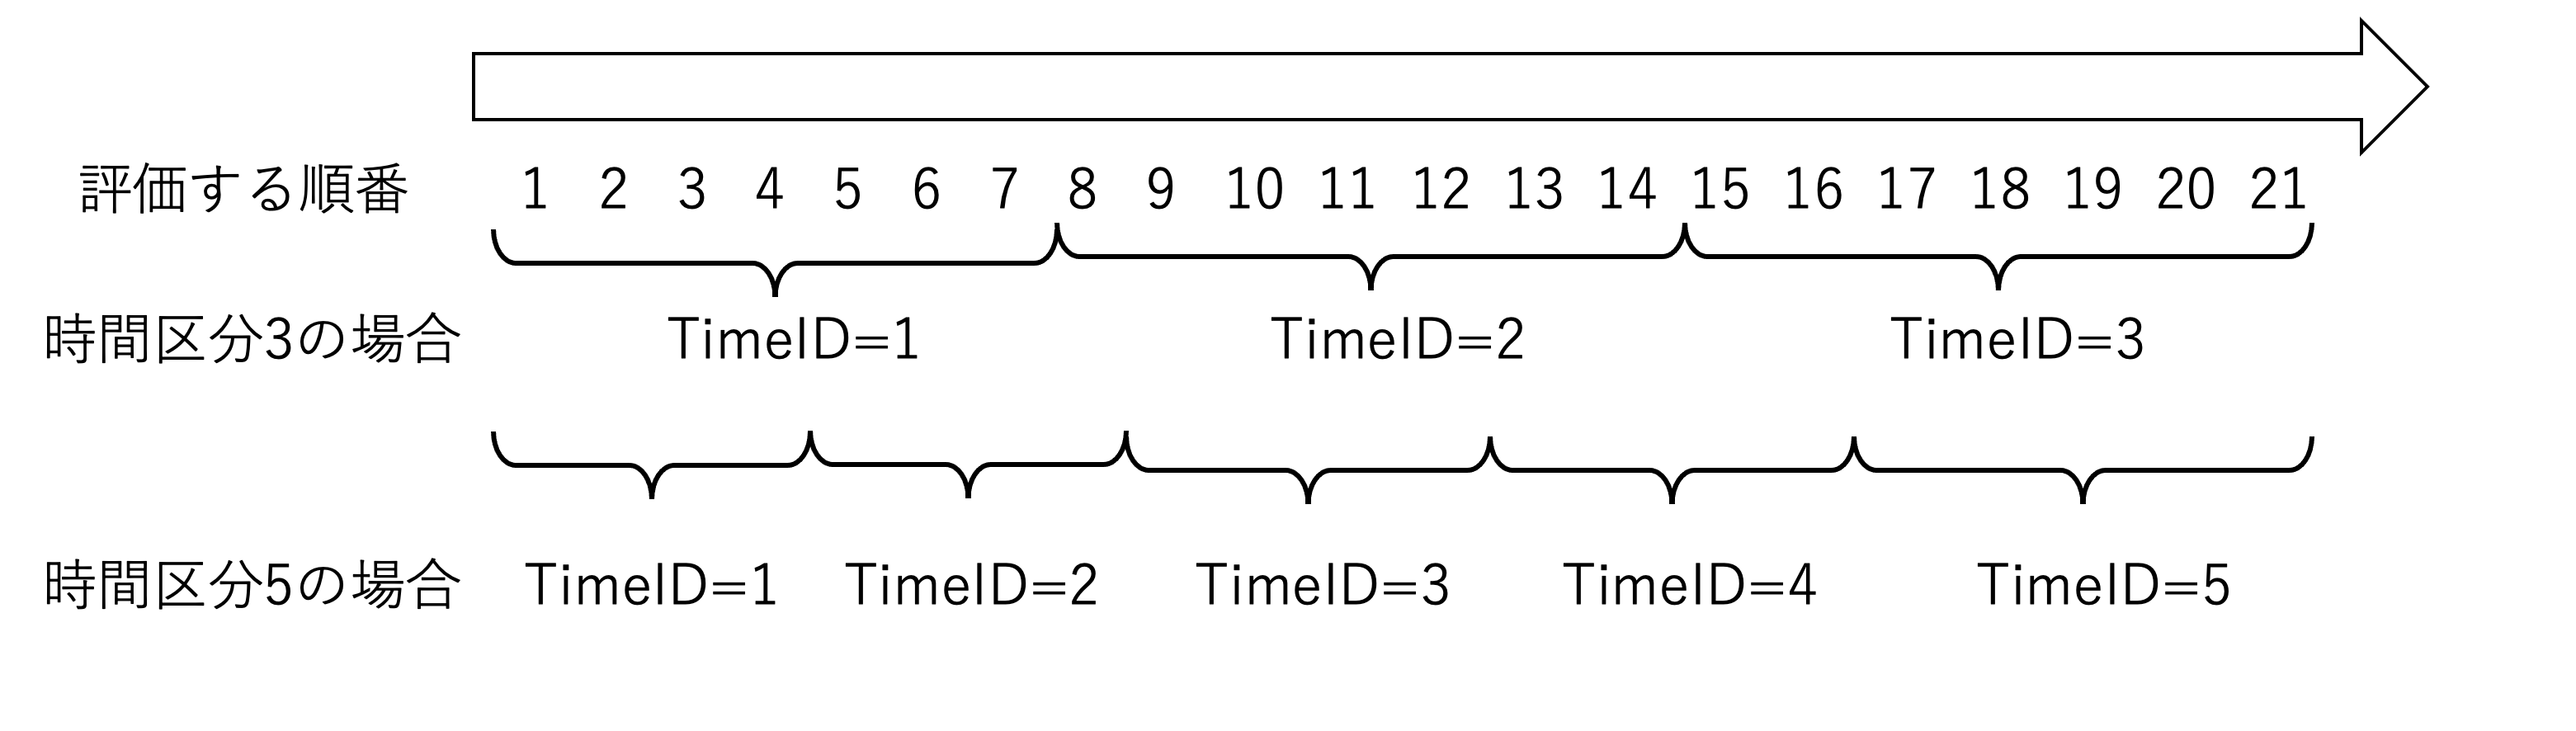
\includegraphics[width=10cm]{img/timeid.png}
\caption{時間区分データのイメージと例}
 \label{timeid}
\end{figure}

\section{評価者ドリフトを考慮したIRT}

Wolfe et. al\cite{Wolfe}は,一般的な多相ラッシュモデルに時間のパラメータを追加したモデルを提案している.このモデルでは,評価者$r$が課題$i$における受検者$j$のパフォーマンスに時間区分$t$において評点$k$を与える確率を次の式で定義する.
\begin{equation}
P_{ijrtk}=\frac{\mathrm{exp}\sum_{m=1}^{k}(\theta_{j}-\beta_{i}-\beta_{r}-\beta_{t}-d_{m})}{\sum_{l=1}^{K}\mathrm{exp}\sum_{m=1}^{l}(\theta_{j}-\beta_{i}-\beta_{r}-\beta_{t}-d_{m})}
\end{equation}
ここで,$\beta_t$は時間区分$t$における全ての評価者の平均的な評価の厳しさを表す.
このモデルは,全ての評価者の特性が同じ傾向で時間変動すると想定しているが,実際には変化の度合いも評価者によって異なる.そこで,評価者ごとの変化の度合いも考慮できるモデルとして,RaudenbushとBryk\cite{Raudenbush}は,評価者の厳しさの安定性を調べるために,時間$t$における評価者$r$の厳しさの変化を反映させるモデルを次の式で提案した.
\begin{equation}
P_{ijrtk}=\frac{\mathrm{exp}\sum_{m=1}^{k}(\theta_{j}-\beta_{i}-\beta_{r} - \pi_{r}t-d_{m})}{\sum_{l=1}^{K}\mathrm{exp}\sum_{m=1}^{l}(\theta_{j}-\beta_{i}-\beta_{r} - \pi_{r}t-d_{m})}
\end{equation}
ここで,$\beta_{r}$は評価者$r$の初期の厳しさ,$\pi_{r}$は評価者$r$の厳しさの変化の傾きを表す.また,$t$は時間区分である.このモデルでは,各評価者の初期の厳しさと,厳しさの傾きが変化し,個々の評価者ごとに結果を得ることができる.重要なのは,時間区分ごとの変化である$\pi_{r}$で,どの評価者が試験サイクルごとに厳しさが変化する傾向があるかを示している.

\section{既存モデルの課題}
本節では,4.2で紹介したモデルが抱える問題点について述べる.

4.2で紹介したモデルは,パフォーマンス評価において,評価者と時間における評価者特性の変化を考慮することが可能である.しかし,このモデルの問題点として次の点が挙げられる.
\begin{enumerate}
  \item 評価者特性の変化を直線的にしかとらえることができない
  \item 評価者の一貫性と各得点に対する基準の差異を考慮できていない.
\end{enumerate}  
以上の問題を解決するため,時間区分ごとの評価者の厳しさを推定できる新しいIRTモデルを次節で提案する.
\newpage
\chapter{提案モデル}
提案モデルでは,受検者$j$のパフォーマンスに, 評価者$r$が時間区分$t$において評点$k$を与える確率$P_{jrtk}$を次式で定義する.なお,本研究では,課題数は1と仮定し,課題パラメータは考慮しないこととする.
\begin{equation}
P_{jrtk}=\frac{\mathrm{exp}\sum{\alpha_r(\theta_{j}-\beta_{rt}-d_{rk})}}{\sum \mathrm{exp}\sum{\alpha_r(\theta_{j}-\beta_{rt}-d_{rk})}}
\end{equation}
\begin{eqnarray}
  \beta_{rt}\sim \mathrm{N}(\beta_{r(t-1)},\sigma)\nonumber\\
  \beta_{r1} \sim \mathrm{N}(0,1)\nonumber\\
  \sigma \sim \mathrm{LN}(-3,0)\nonumber
\end{eqnarray}
ここで,$\alpha_{r}$は評価者$r$の一貫性,$\theta_{j}$は受検者$j$の能力,$\beta_{rt}は$評価者$r$の時間区分$t$における厳しさ,$d_{rk}$は評価者$r$からスコア$k$を得る困難度を示すステップパラメータである.
また,$\mathrm{N}(\mu,\sigma)$は平均$\mu$,標準偏差$\sigma$の正規分布を表し,$\mathrm{LN}(\mu,\sigma)$は平均$\mu$,標準偏差$\sigma$の対数正規分布を表す.

提案モデルでは,$\beta_{rt}$が$\beta_{r(t-1)}$を平均とする正規分布に従うと仮定している.
ただし,ある時間区分における評価者の厳しさは直前の時間区分時点での厳しさから一般には大きく変化しないと考えられる.
そこで,ここでは$\beta_{rt}$が従う分布の標準偏差$\sigma$が小さくなるように,$\sigma$の事前分布に$\mathrm{LN}(−3,0)$を採用している.

また,モデルの識別性のために,$\theta_{j}\sim N(0,1),\prod_{r}\alpha_r=1,d_{r1}=0,\sum_{k=2}^{K}d_{rk}=0$を仮定する.

提案モデルの利点として,以下の点が挙げられる.
\begin{enumerate}
  \item 時間区分ごとの評価者特性の変化をより柔軟に推定することができるため,データへのモデル適合度が向上し,モデルの性能が改善する.
  \item 評価者ごとの一貫性の差異,及び各段階得点に対する基準の差異をより柔軟に考慮できるため,データへのモデル適合度が向上し,モデルの性能が改善する.
\end{enumerate}
これらの特徴は,第4章で述べた既存モデルの問題点を解決することができるものである.

\section{パラメータの解釈}
本節では,提案モデルの評価観点パラメータと評価者パラメータの解釈について説明する.
このために,カテゴリ数$K=5$において,表\ref{iccparam}のパラメータを所与とした時の項目反応曲線(ICC: Item Characteristic Curve)を図\ref{icc}に示す.なお,表\ref{iccparam}では,パラメータの意味が理解しやすい例を示すために,モデルの識別性の条件式を必ずしも満たさないパラメータ値を用いているが,条件式を満たす値でも解釈は同様である.各図は,横軸が受検者の能力$\theta_j$を表し,縦軸が各評点への反応確率$P_{ijrtk}$を表す.図\ref{icc}から,いずれのICCにおいても,能力が低いほど低い評点を得る確率が高くなり,能力が高いほど高い評点を得る確率が高くなっていることがわかる.

ここで,表\ref{icc}の(a),(b),(c)は$\beta_{rt}$以外のパラメータ一定のもとで$\beta_{rt}$を変更した場合に対応し,(a)と(d),(e),(f)は$\beta_{rt}$が一定のもとで他のパラメータを変更した場合に対応している.まず,時間区分に関わるパラメータの解釈を説明するために(a)を基準に(b)と(c)を比較する.

(b)は(a)と比較して$\beta_{rt}$の値が大きくなっている.これは,時間区分1の時よりも時間区分2の時の方が評価者の厳しさが大きくなっているという意味である.(b)のICCでは,(a)と比べて全体的に右に移動していることが確認できる.これは,$\beta_{rt}$が大きくなっている時間区分では,良い評価を得るためにより高い能力が必要となっていることを示している.

(c)は(a)と比較して$\beta_{rt}$が小さくなっている.これは,時間区分1の時よりも時間区分3の時の方が評価者の厳しさが小さくなっているという意味である.(c)のICCでは,(a)と比べて全体的に左に移動していることが確認できる.これは,$\beta_{rt}$が小さくなっている時間区分では,良い評価を得るために要求される能力値が低くなっていることを示している.提案モデルでは,このように各時間区分における評価者の厳しさを,評価者ごとに表現する.

次に,評価者特性の解釈を説明するために(a)を基準に(d),(e),(f)を比較する.

(d)は(a)と比較して,$d_{r3}$と$d_{r4}$の差が小さく,$d_{r4}$と$d_{r5}$の差が大きくなっている.このパラメータは, 隣接する$d_{rk+1} − d_{rk}$の差が大きくなるほど, 評点$k$と評点$k+1$の基準の乖離が大きいことを意味する.(a)のICCと比較すると,評点4への反応確率が高くなる能力値の範囲が広く,評点3への反応確率が高くなる能力値の範囲が狭くなっている.提案モデルでは,このように各カテゴリに対する評価基準を,評価者ごとに表現する.

(e)は(a)と比較して,$\alpha_r$の値が大きくなっている.ICCを比べると,(a)よりも曲線の勾配が大きくなっている.これは,一貫性の高い評価者は,受検者の能力と相関した評点を与えるとともに,同等の能力の受検者には安定して同一の評点を与える傾向が強いことを表現している.

(f)は(a)と比較して,$\alpha_r$の値が小さくなっている.ICCを比べると,(a)よりも曲線の勾配が小さくなっている.これは,一貫性の低い評価者は,評価にばらつきがあり,受検者の能力と評点の相関が小さくなることを示している.
\begin{table*}[t]
\begin{center}
\caption{図5.1で使用するパラメータ}
\setlength{\tabcolsep}{5.pt}
\begin{tabular}{cccccccccccccc}  
\bhline{1pt}
  & 評価者& 時間区分& & $\alpha_1$ & $\beta_{rt}$ & $d_{r1}$ & $d_{r2}$ & $d_{r3}$ & $d_{r4}$ & $d_{r5}$\\
\bhline{1pt}
  &評価者1  & 時間区分1 & & 1.0 & 0.0  & 0.0 & -1.0 & 0.0 & 0.5 & 1.0\\
  & & 時間区分2 & & 1.0 & 0.5  & 0.0 & -1.0 & 0.0 & 0.5 & 1.0\\
  & & 時間区分3 & & 1.0 & -0.5  & 0.0 & -1.0 & 0.0 & 0.5 & 1.0\\
\bhline{1pt}
  & & & & $\alpha_r$ & $\beta_{rt}$ & $d_{r1}$ & $d_{r2}$ & $d_{r3}$ & $d_{r4}$ & $d_{r5}$\\
\bhline{1pt}
  & 評価者2&  時間区分1 & & 1.0 & 0.0  & 0.0 & -1.0 & 0.0 & 0.2 & 1.0\\
  &評価者3  & 時間区分1 & & 2.0 & 0.0  & 0.0 & -1.0 & 0.0 & 0.5 & 1.0\\
  & 評価者4& 時間区分1 & & 0.5 & 0.0  & 0.0 & -1.0 & 0.0 & 0.5 & 1.0\\
\bhline{1pt}
\end{tabular}
\label{iccparam}
\end{center}
\end{table*}
\begin{center}
  \begin{figure}[]
  \begin{minipage}[b]{0.3\linewidth}
    \centering
    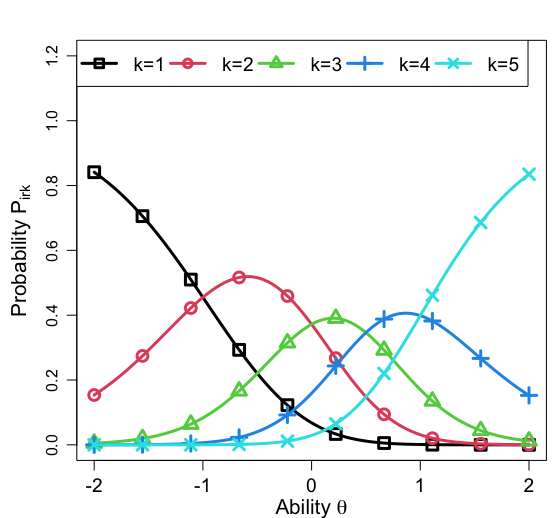
\includegraphics[keepaspectratio,scale=0.22]{img/icc1.png}
    \subcaption{評価者1,時間区分1}\label{1}
  \end{minipage}
  \begin{minipage}[b]{0.3\linewidth}
    \centering
    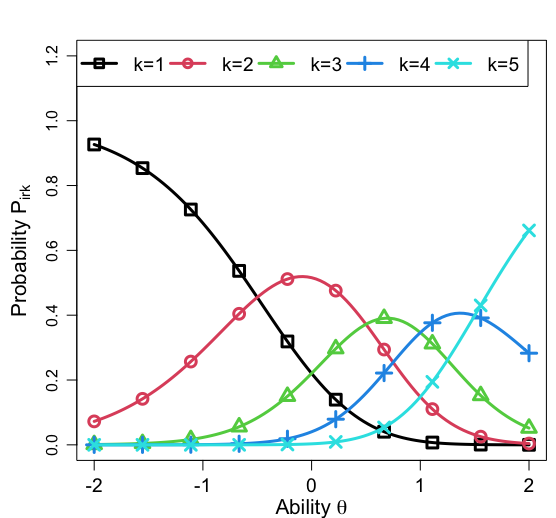
\includegraphics[keepaspectratio,scale=0.22]{img/icc2.png}
    \subcaption{評価者1,時間区分2}\label{2}
  \end{minipage}
  \begin{minipage}[b]{0.3\linewidth}
    \centering
    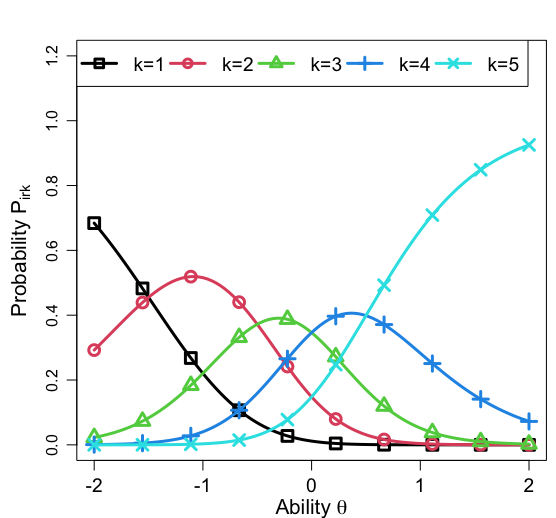
\includegraphics[keepaspectratio,scale=0.22]{img/icc3.png}
    \subcaption{評価者1,時間区分3}\label{3}
  \end{minipage}\\
  \begin{minipage}[b]{0.3\linewidth}
    \centering
    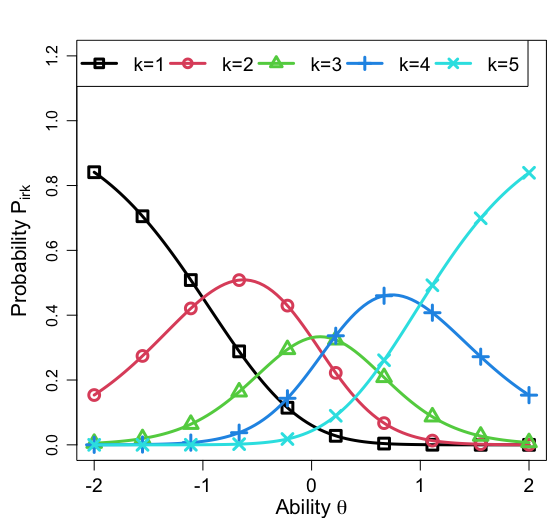
\includegraphics[keepaspectratio,scale=0.22]{img/icc4.png}
    \subcaption{評価者2,時間区分1}\label{4}
  \end{minipage}
  \begin{minipage}[b]{0.3\linewidth}
    \centering
    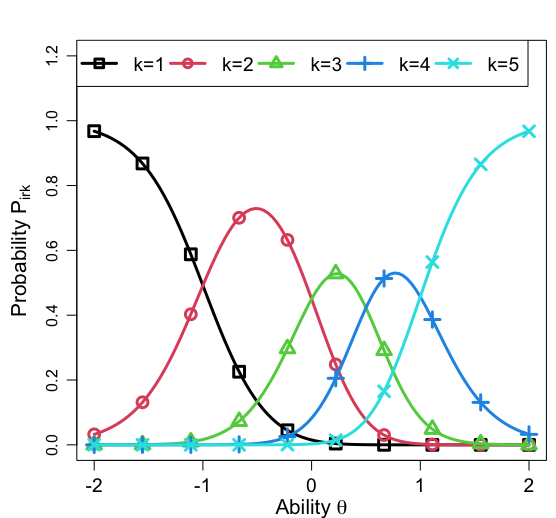
\includegraphics[keepaspectratio,scale=0.22]{img/icc5.png}
    \subcaption{評価者3,時間区分1}\label{5}
  \end{minipage}
  \begin{minipage}[b]{0.3\linewidth}
    \centering
    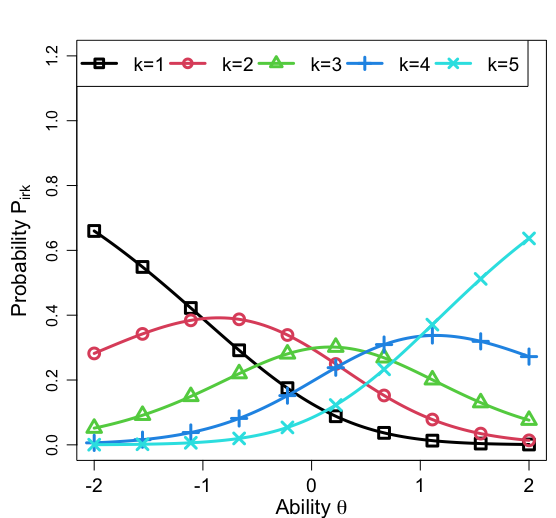
\includegraphics[keepaspectratio,scale=0.22]{img/icc6.png}
    \subcaption{評価者4,時間区分1}\label{6}
  \end{minipage}\\
  \caption{表\ref{iccparam}のパラメータを適用した場合のICC}\label{icc}
  \end{figure}
\end{center}
\section{パラメータ推定手法}
本節では提案モデルのパラメータ推定手法について述べる.IRTのパラメータ推定手法としては,EMアルゴリズムを用いた周辺最尤推定法やニュートンラフソン法による事後確率最大化推定法が広く用いられてきた.一方で,本研究で扱うような複雑なIRTモデルの場合には,マルコフ連鎖モンテカルロ(MCMC:Markov Chain Monte-Carlo)を用いた期待事後確立推定法が高精度であることが知られている\cite{IRTUtoUeno,norm}.

IRTにおけるMCMCアルゴリズムとしては,メトロポリタンヘイスティングスとギブスサンプリングを組み合わせたアルゴリズム(Gibbs/MH)\cite{IRTUtoUeno,Patz,BiasUsami}が利用されてきた.このアルゴリズムは,単純で実装が容易である反面,目標分布への収束が遅いという問題がある\cite{Hoffman,Giroami}.

Gibbs/MHより効率の良いMCMCアルゴリズムとして,ハミルトニアンモンテカルロ(HMC)が知られている\cite{Rosenthal}.HMCでは,ステップサイズとシミュレーション長という2つの決定変数を適切に選択することで,自己相関の低い良質なサンプルを得ることができ,高速に目標分布に収束することが知られている\cite{Hoffman,Neal}.近年では,HMCの決定変数をサンプリングの過程で最適化できるNo-U-TrunSampler(NUT)\cite{Hoffman}と呼ばれる手法が提案されている.NUTによるMCMCは,Stan\cite{stan}と呼ばれるライブラリの整備により,さまざまな数理モデルに容易に適用できるようになったため,IRTを含む様々な統計・機械学習モデルの推定に近年広く利用されている\cite{Luo,Jiang,Matsura}.

以上より,本研究では提案モデルのパラメータ推定手法としてStanを用いたNUTによるMCMC法を用いる.実装はRStan\cite{rstan}を用いて行った.提案モデルのStanコードは付録に示した.パラメータの事前分布は$\theta_{j},d_{rk},\mathrm{log}\alpha_{r},\beta_{r1}\sim N(0.0,1.0^{2})$とした.ここで,$N(\mu,\sigma^2)$は平均$\mu$,標準偏差$\sigma$の正規分布を表す.本研究では,MCMCのバーンイン期間は1000とし,1000$\sim$2000時点までの1000サンプルを用いる.

\newpage
\chapter{シミュレーション実験}

本節では,MCMCアルゴリズムによる提案モデルと,式(4.2)の既存モデル(以下では「既存モデル」と書く)のパラメータ推定精度をシミュレーション実験により評価する.実験手順は以下の通りである.
\begin{enumerate}
\item パラメータの真値を,モデルの分布に従って生成する
\item 手順1で生成したパラメータを用いて,データを生成する
\item 手順2で生成したデータからパラメータ推定を行う
\item 手順3で得られたパラメータ推定値と手順1で生成したパラメータ真値において,平均平方二乗誤差(RMSE)とバイアスを求める
\item 以上を5回繰り返し実行し,RMSEとバイアスの平均値を求める
\end{enumerate}
上記の実験を,受検者数$J=60$,$90$,$120$,評価者数$R=10$,$15$,時間区間$T=3$,$5$,$10$の場合において行った.カテゴリ数は$K=5$とした.

\section{パラメータ真値}
この実験で使用するパラメータの真値について説明する.
$\beta_{rt}$以外のパラメータの真値は,主に5章にて説明した分布に従って生成したが,一方で,$\beta_{rt}$については個別でパターンを作成し,生成するようにした.作成したパターンとしては,
\begin{description}
\item [採点中に一回厳しさが変化する]\mbox{}\\
初期値$\beta_{r1}$を正規分布に従う乱数で生成し,採点の真ん中のタイミング(T=10ならt=5からt=6に変わる時)で$\beta_{r1}+\delta$に変化させる.なお,$\delta$は$N(0,0.2)$に従う乱数である.
\item [採点中に時間区分ごとに厳しさがほとんど変化しない]\mbox{}\\
初期値$\beta_{r1}$を正規分布に従う乱数で生成し,次の時間区分からは$\beta_{r1}+\delta_t$となる.なお,$\delta_t$は$N(0,0.01)$に従う0に近い値を取る乱数であり,$t$が変わるごとに変化する.
\item [採点中に厳しさが線形変化する]\mbox{}\\
初期値$\beta_{r1}$を正規分布に従う乱数で生成し,次の値からは$\delta_r \times t +\beta_{r1}$となる.なお,$\delta_r$は$N(0,0.01)$に従う乱数である.
\end{description}
の3種類を作成した.これらのパターンは,それぞれ全評価者数の3分の1ずつになるように作成した.
\section{実験結果}
提案モデルの実験結果を表\ref{parameters_recovery1}に示す.表\ref{parameters_recovery1}から,全パラメータのRMSEの平均値は$0.2\sim0.3$程度となり,パラメータ別の最大値でも0.38までに収まっていることがわかる.0.2や0.38という値は,標準正規分布に従うサンプルの99.73\%が含まれる範囲(-3$\sim$3)の3.3\%と6.3\%に相当し,十分に小さい値と解釈できる.また,関連研究\cite{UtoUeno,YagiUto,IRTUtoUeno}と同様に,受検者数・評価者数の増加に伴い推定精度が改善する傾向も読み取れる.時間区分数の増加に伴って推定制度が改善する傾向は読み取れないが,これは時間区分数の増加はサンプル数が増えるわけではなく,データの中身が変化するだけであるからと考えられる.バイアスの平均については,いずれのパラメータも0に非常に近い値を示しており,系統的な過大(または過少)推定の傾向もないことが確認できる.また,MCMCの収束を示すGelman-Rubin の収束判定指標$ \hat{R} $\cite{RhatRubin,RhatCarlin}を確認したところ,すべての場合で一般的な収束判定基準値である1.1を下回っていた.

また,$\beta_{rt}$のパターンごとの推定結果の例を図\ref{beta_rt_recovery}に示す.実線が作成したパラメータ真値,波線が推定したパラメータである.このグラフより,作成した真値にある程度従って,パラメータが推定されていることがわかる.

以上の結果から, MCMCにより提案モデルのパラメータを適切に推定できることが確認できた.


また,表\ref{parameters_recovery2}に既存モデルの実験結果を示す.
表\ref{parameters_recovery2}から,提案モデルと比べるとRMSE,バイアスともにやや悪い傾向があるが,全体としては受検者数や評価者数の増加に伴う推定精度の改善傾向は確認でき,適切に推定されていると言える.
また,収束判定指標の$\hat{R} $\cite{RhatRubin,RhatCarlin}も全て1.1を下回っており,MCMCの収束も確認できた.
以上の結果から,MCMCにより既存モデルのパラメータを適切に推定できることが確認できた.

\begin{table*}[tb]
\begin{center}
\caption{提案モデルのパラメータ・リカバリ実験の結果}
\setlength{\tabcolsep}{5.pt}
\begin{tabular}{cccccccccccccc}  
\bhline{1pt}
\multirow{2}{*}{$J$} & \multirow{2}{*}{$R$} & \multirow{2}{*}{$T$}  && \multicolumn{4}{c}{RMSE} &&   \multicolumn{4}{c}{BIAS}  \\
\cline{5-8}\cline{10-13}
  & & & & $\theta$ & $\alpha_r$ & $\beta_{rt}$ & $d_{rk}$ &  & $\theta$ & $\alpha_r$ & $\beta_{rt}$ & $d_{rk}$ \\
\bhline{1pt}
60 & 10 & 3  && 0.28 & 0.23 & 0.19 & 0.34 && -0.01 & 0.01 & -0.01 & 0.00 \\
   &    & 5  && 0.29 & 0.26 & 0.25 & 0.37 && 0.00  & 0.02 & -0.03 & 0.00 \\
   &    & 10 && 0.29 & 0.23 & 0.23 & 0.37 && 0.00  & 0.01 & 0.00  & 0.00 \\
\cline{2-14}
   & 15 & 3  && 0.23 & 0.27 & 0.24 & 0.38 && 0.01  & 0.01 & 0.01  & 0.00 \\
   &    & 5  && 0.22 & 0.22 & 0.23 & 0.36 && 0.00  & 0.01 & 0.02  & 0.00 \\
   &    & 10 && 0.26 & 0.27 & 0.31 & 0.38 && -0.02 & 0.01 & -0.04 & 0.00 \\
\hline
90 & 10 & 3  && 0.26 & 0.23 & 0.14 & 0.30 && -0.01 & -0.02 & -0.02 & 0.00 \\
   &    & 5  && 0.26 & 0.25 & 0.16 & 0.30 && 0.01  & 0.02  & 0.03  & 0.00 \\
   &    & 10 && 0.29 & 0.27 & 0.23 & 0.31 && 0.00  & 0.03  & 0.02  & 0.00 \\
\cline{2-14}
& 15 & 3  && 0.21 & 0.21 & 0.17 & 0.32 && 0.03  & 0.01 & 0.06  & 0.00 \\
&    & 5  && 0.24 & 0.21 & 0.21 & 0.34 && 0.00  & 0.00 & -0.01 & 0.00\\
&    & 10 && 0.23 & 0.24 & 0.26 & 0.35 && -0.01 & 0.02 & -0.01 & 0.00\\
\hline
120 & 10 & 3  && 0.26 & 0.19 & 0.15 & 0.27 && -0.01 & 0.01 & 0.00  & 0.00 \\
    &    & 5  && 0.28 & 0.21 & 0.18 & 0.32 && 0.00  & 0.01 & -0.01 & 0.00 \\
    &    & 10 && 0.28 & 0.20 & 0.25 & 0.29 && -0.01 & 0.00 & -0.03 & 0.00\\
\cline{2-14}
& 15 & 3  && 0.22 & 0.19 & 0.13 & 0.24 && 0.02 & 0.00 & 0.03 & 0.00 \\
&    & 5  && 0.23 & 0.17 & 0.18 & 0.31 && 0.02 & 0.02 & 0.05 & 0.00 \\
&    & 10 && 0.24 & 0.20 & 0.26 & 0.30 && 0.00 & 0.01 & 0.00 & 0.00 \\
\hline
\multicolumn{4}{c}{Avg.}   &  0.26 & 0.24 & 0.24 & 0.34 &  & 0.01 & 0.01 & 0.01 & 0.00 & \\
\bhline{1pt}
\end{tabular}
\label{parameters_recovery1}
\end{center}
\end{table*}



\begin{table*}[tb]
  \begin{center}
  \caption{既存モデルのパラメータ・リカバリ実験の結果}
  \setlength{\tabcolsep}{5.pt}
  \begin{tabular}{cccccccccccccc}  
  \bhline{1pt}
  \multirow{2}{*}{$J$} & \multirow{2}{*}{$R$} & \multirow{2}{*}{$T$}  && \multicolumn{4}{c}{RMSE} &&   \multicolumn{4}{c}{BIAS}  \\
  \cline{5-8}\cline{10-13}
    & & & & $\theta$ & $\beta_r$ & $\pi_{r}$ & $d_{k}$ &  & $\theta$ & $\beta_r$ & $\pi_{r}$ & $d_{k}$ \\
  \bhline{1pt}
  60  & 10 & 3  &  & 0.32 & 0.41 & 0.50 & 0.08 &  & -0.06 & 0.00 & -0.07 & 0.00 \\
    &    & 5  &  & 0.34 & 0.57 & 0.67 & 0.10 &  & 0.12  & 0.00 & 0.22  & 0.00 \\
    &    & 10 &  & 0.35 & 0.47 & 0.64 & 0.10 &  & 0.06  & 0.00 & 0.05  & 0.00 \\
  \cline{2-14}
  & 15 & 3  &  & 0.28 & 0.58 & 0.57 & 0.07 &  & -0.06 & 0.00 & -0.03 & 0.00 \\
  &    & 5  &  & 0.25 & 0.50 & 0.57 & 0.08 &  & -0.03 & 0.00 & -0.04 & 0.00 \\
  &    & 10 &  & 0.28 & 0.47 & 0.72 & 0.08 &  & 0.04  & 0.00 & 0.01  & 0.00 \\
  \hline
  90  & 10 & 3  &  & 0.32 & 0.50 & 0.57 & 0.06 &  & -0.07 & 0.00 & -0.03 & 0.00 \\
  &    & 5  &  & 0.31 & 0.47 & 0.55 & 0.07 &  & -0.03 & 0.00 & -0.11 & 0.00 \\
  &    & 10 &  & 0.32 & 0.52 & 0.61 & 0.10 &  & -0.02 & 0.00 & -0.03 & 0.00 \\
  \cline{2-14}
  & 15 & 3  &  & 0.26 & 0.42 & 0.51 & 0.08 &  & -0.05 & 0.00 & -0.07 & 0.00 \\
  &    & 5  &  & 0.31 & 0.78 & 0.69 & 0.08 &  & 0.00  & 0.00 & -0.08 & 0.00 \\
  &    & 10 &  & 0.28 & 0.53 & 0.59 & 0.08 &  & 0.04  & 0.00 & -0.08 & 0.00 \\
  \hline
  120 & 10 & 3  &  & 0.31 & 0.54 & 0.59 & 0.07 &  & 0.10  & 0.00 & 0.07  & 0.00 \\
  &    & 5  &  & 0.33 & 0.45 & 0.53 & 0.07 &  & 0.05  & 0.00 & 0.08  & 0.00 \\
  &    & 10 &  & 0.32 & 0.45 & 0.61 & 0.08 &  & -0.02 & 0.00 & -0.08 & 0.00 \\
  \cline{2-14}
  & 15 & 3  &  & 0.27 & 0.48 & 0.46 & 0.06 &  & -0.03 & 0.00 & -0.11 & 0.00 \\
  &    & 5  &  & 0.27 & 0.46 & 0.58 & 0.07 &  & -0.01 & 0.00 & 0.01  & 0.00 \\
  &    & 10 &  & 0.28 & 0.51 & 0.64 & 0.07 &  & -0.02 & 0.00 & -0.05 & 0.00\\
  \hline
  \multicolumn{4}{c}{Avg.}   &  0.30 & 0.51 & 0.60 & 0.07 &  & 0.00 & 0.00 & -0.02 & 0.00 & \\
  \bhline{1pt}
  \end{tabular}
  \label{parameters_recovery2}
  \end{center}
\end{table*}
\clearpage
\begin{figure}[tb]
 \begin{minipage}[tb]{0.3\linewidth}
  \centering
  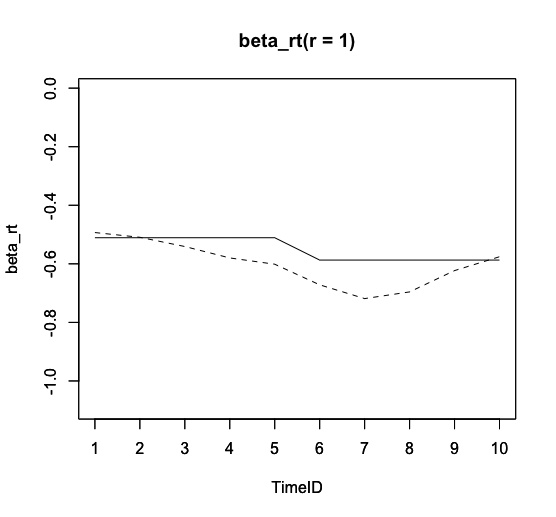
\includegraphics[keepaspectratio,scale=0.25]{img/beta_rt_param_1.png}
  \subcaption{パターン1}\label{ICC1}
 \end{minipage}
 \begin{minipage}[tb]{0.3\linewidth}
  \centering
  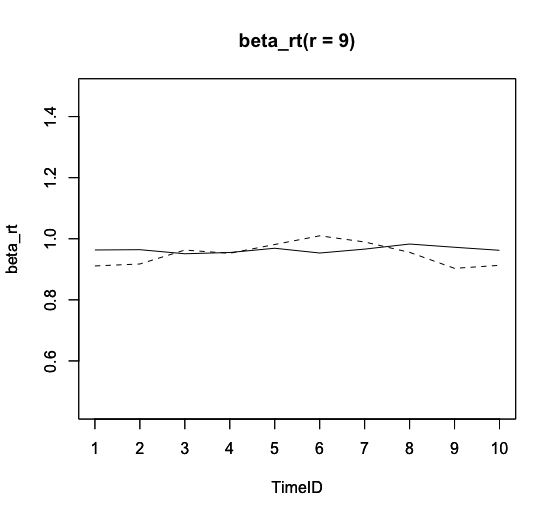
\includegraphics[keepaspectratio,scale=0.25]{img/beta_rt_param_9.png}
  \subcaption{パターン2}\label{ICC2}
 \end{minipage}
 \begin{minipage}[tb]{0.3\linewidth}
  \centering
  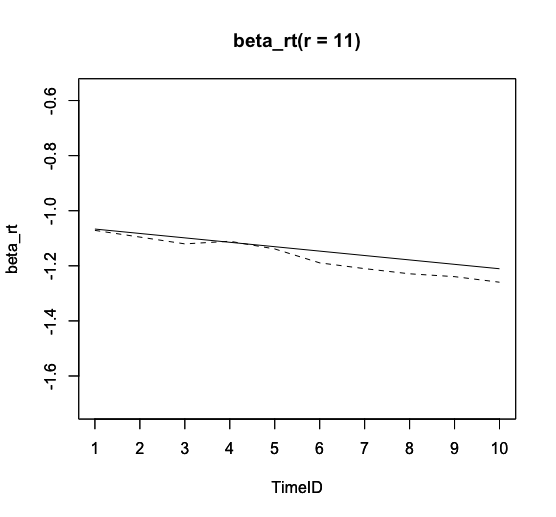
\includegraphics[keepaspectratio,scale=0.25]{img/beta_rt_r_11.png}
  \subcaption{パターン3}\label{ICC3}
 \end{minipage}\\
 \caption{$\beta_{rt}$の推定例}\label{beta_rt_recovery}
\end{figure}

\newpage
\chapter{実データ実験}
本章では,実データの適用を通して,提案モデルの有効性を評価する.

本研究では,134名分のエッセイ課題を,16名の評価者が5段階得点で採点したデータを使用する.
採点は4日に分け,日ごとに全体の1/4ずつ採点するように指示した.以降では日ごとに時間区分1,2,3,4として扱う.
全16名の被験者のうち,6人には採点の際に指示を与え,人為的に評価者バイアスのあるデータを作成するようにした.これらの6人を評価者A,B,C,D,E,Fとすると,それぞれに与えた指示は以下の通りである.

\begin{description}
  \item [評価者A]日ごとにだんだん厳しくなるように採点する
  \item [評価者B]日ごとにだんだん優しくなるように採点する
  \item [評価者C]日によって厳しさを変えて採点する.具体的には,2日目は1日目より厳しく,3日目は1日目より甘く,4日目は2日目よりさらに厳しくなるように採点する.
  \item [評価者D]使用する得点に偏りを持たせ,2,3,4点を多く使用するように採点する
  \item [評価者E]使用する得点に偏りを持たせ,1,3,5点を多く使用するように採点する
  \item [評価者F]採点基準を用いずに採点する
\end{description}

本研究では,このように収集したデータに対して提案モデルを適用する.
\section{評価者特性}
実データから推定された評価者パラメータを表\ref{param}に示す.
また,$\beta_{rt}$の推定結果をグラフにしたものを図\ref{beta_rt_data_img}に示す.縦軸が$\beta_{rt}$,横軸が時間区分である.色がついているものは,前述した指示を与えた評価者のデータであり,黒が評価者A,赤が評価者B,緑が評価者C,青が評価者D,水色が評価者E,紫が評価者Fである.
これを見ると,指示を与えた評価者は,その指示通りの評価者バイアスを示していることを推定できている.また,指示を与えていない評価者でも,評価者ごとにパラメータの変化を推定できていることがわかる.例えば$r=2$の評価者は時間区分1から2に変化するときに厳しさが大幅に上昇し,そのあとは緩やかに低下していることがわかる.
また,評価者Dと評価者Eの評価者パラメータから作成したICCを表\ref{ICC_DE}に示す.これを見ると,どちらも多く使うように指示した得点を多く使用していることがデータから推定できていることがわかる.
また,$\alpha_r$の値を評価者ごとに比べると,評価者ごとに一貫性に差があることがわかる.
さらに,評価者ごとにステップパラメータ$d_{rk}$の値に差があることが読み取れる.

以上のことから,提案モデルでは,時間区分ごとの評価者の厳しさの変化と,評価者ごとの一貫性,得点の使用傾向の違いを推定することができているとわかる.
\begin{table*}[tb]
\begin{center}
\caption{パラメータ推定値}
\setlength{\tabcolsep}{5.pt}
\begin{tabular}{ccccccccccccccccccc}  
\bhline{1pt}
& & $r$ & & $\alpha_r$ & $\beta_{r1}$ & $\beta_{r2}$ & $\beta_{r3}$ &$\beta_{r4}$ & $d_{r1}$ &  $d_{r2}$ & $d_{r3}$ & $d_{r4}$ & $d_{r5}$  \\
\bhline{1pt}
 &  & 1  &  & 0.71 & -0.48  & -0.46 & -0.46 &-0.72 & 0.00  & -2.13 & -0.23 & 0.63 & 1.73\\
 &  & 2  &  & 1.07 & -0.03  & 0.28  & 0.25  & 0.21 & 0.00  & -0.86 & -0.51 & 0.54 & 0.83 \\
 &  & 3  &  & 1.57 & -0.87  & -0.92  & -1.02  & -0.90 & 0.00 & -0.92 & -1.26  & 0.39 & 1.79 \\
 &  & 4  &  & 0.97 & -0.58  & -0.90  & -0.56 & -0.35 & 0.00 & -1.62 & -1.27  & 0.77 & 2.12 \\
 &  & 5  &  & 1.14 & -0.14 & -0.23 & -0.23 & -0.33 & 0.00 & -2.30 & -0.28  & 0.80 & 1.78\\
 &  & 6  &  & 0.93 & 0.47 & 0.14 & -0.05 & 0.04 & 0.00 & -1.63 & -0.64  & 0.48 & 1.80\\
 &  & 7  &  & 0.82 & -0.29  & -0.43 & -0.47 & -0.40 & 0.00 & -1.18 & -0.09  & 0,71 & 0.56 \\
 &  & 8  &  & 1.32 & 0.03 & 0.35 & 0.37 & 0.32 & 0.00 & -1.41 & -0.65  & 0.75 & 1.31 \\
 &  & 9  &  & 0.77 & -0.82 & -0.84 & -0.73 & -0.83 & 0.00 & -1.00 & -0.45 & 0.47 & 0.98 \\
 &  & 10 &  & 1.00 & -0.31 & -0.51 & -0.64 & -0.49 & 0.00 & -1.52 & -0.13 & 0.38 & 1.26 \\
 &  & 11(評価者A) &  & 1.16 & -1.05 & -0.85 & -0.03 & 0.22 & 0.00 & -1.66 & -0.66 & 0.92 & 1.40 \\
 &  & 12(評価者B) &  & 1.23 & 0.68 & 0.28 & 0.16 & -0.02 & 0.00 & -0.96 & -0.10 & 0.21 & 0.84 \\
 &  & 13(評価者C) &  & 1.02 & -0.27 & 0.01 & -0.45 & 0.08 & 0.00 & -1.08 & -0.70 & 0.73 & 1.05\\
 &  & 14(評価者D) &  & 0.68 & -0.09  & -0.15 & -0.18 & -0.15 & 0.00 & -1.69 & -0.71 & 0.42 & 1.97 \\
 &  & 15(評価者E) &  & 1.16 & -0.22 & -0.23 & -0.22 & -0.42 & 0.00 & 0.19 & -1.20  & 1.37 & -0.36 \\
 &  & 16(評価者F) &  & 0.87 & -0.11 & 0.05 & -0.08 & -0.03 & 0.00 & -0.90 & -0.46 & 0.06 & 1.29 \\
\bhline{1pt}
\end{tabular}
\label{param}
\end{center}
\end{table*}

\begin{figure}[tb]
  \begin{center}
  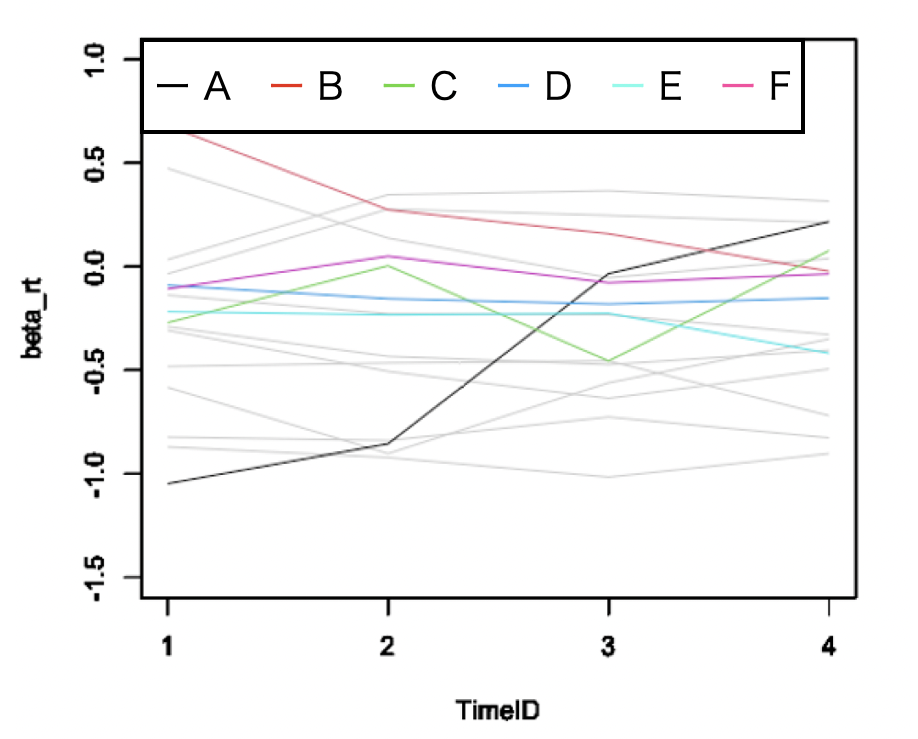
\includegraphics[keepaspectratio, scale=0.5]{img/data_img2.png}
 \caption{$\beta_{rt}$の推定結果}\label{beta_rt_data_img}
\end{center}
\end{figure}


\begin{figure}[tb]
\centering
 \begin{minipage}[b]{0.4\linewidth}
  \centering
  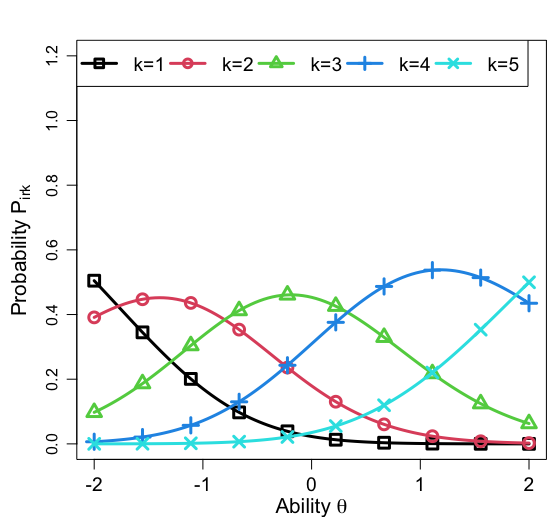
\includegraphics[keepaspectratio,scale=0.25]{img/ICC_r14.png}
  \subcaption{評価者D}\label{D}
 \end{minipage}
 \begin{minipage}[b]{0.4\linewidth}
  \centering
  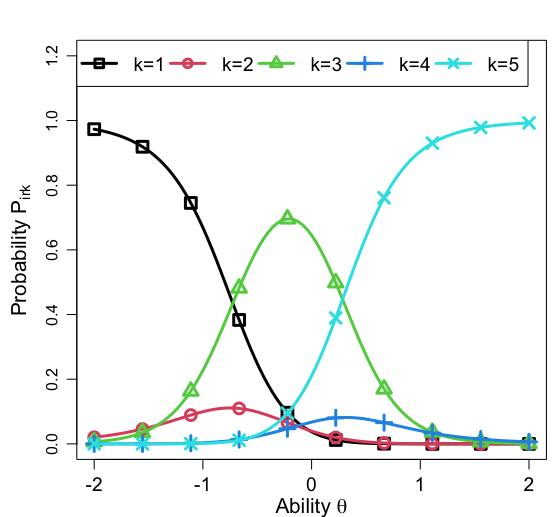
\includegraphics[keepaspectratio,scale=0.25]{img/ICC_r15.png}
  \subcaption{評価者E}\label{E}
 \end{minipage}
 \caption{指示を与えた評価者のICC}\label{ICC_DE}
\end{figure}

\section{情報量基準におけるモデル比較}
本節では,提案モデルの性能を評価するために,\textbf{4.}で紹介した既存モデルとの情報量規準による性能比較を行う.

また,既存モデルから提案モデルへのいくつかの変更点の中で,どの変更が効果を持っていたかを確認するために,以下の3つのモデルとの比較を行う.

\begin{description}
\item [比較モデル1]提案モデルにおいて$d_{rk}$を$d_k$に入れ替えたモデル
\item [比較モデル2]提案モデルにおいて$\beta_{rt}$を$\beta_{r} - \pi_{r}t$に置き換えたモデル
\item [比較モデル3]提案モデルにおいて$\alpha_r$を抜いたモデル
\end{description}

ここでは, MCMCにより各モデルのパラメータを推定し,得られた推定値を用いて情報量規準を求めた.情報量規準にはMCMCのパラメータサンプルから算出できるWAIC(Widely Applicable Information Criterion)とWBIC(Widely Applicable Bayesian Information Criterion)を用いた.ここで,WAICは汎化誤差(まだ手に入れていないデータを予測した時の誤差)の近似であり,将来のデータの予測に優れたモデルを選択する規準である.他方で,WBICは周辺尤度の近似であり,データを生成した真のモデルを漸近的に選択できる基準である.どちらの場合も,値が小さい方が適したモデルであるということを示す.

今回は,全ての評価者データを使用した場合と,指示を与えた評価者を除外した場合に分けて情報量基準を求め,その結果をそれぞれ表\ref{WAIC1},\ref{WAIC2}に示す.

表\ref{WAIC1}と\ref{WAIC2}から,WAICの最小値を比較すると,提案モデルが最適モデルとして選択されたことが確認できる.
また,提案モデルと比較モデル1の結果を比較すると,提案モデルの方がWAICの値が小さいことから,ステップパラメータを評価者に依存させたことによって,提案モデルの性能が向上していることがわかる.加えて,提案モデルと比較モデル2の結果を比較すると,提案モデルの方がWAICの値が小さいことから,時間区分ごとにおける評価者特性を考慮できるようにしたことで,提案モデルの性能が向上していることがわかる.さらに,提案モデルと比較モデル3についても,提案モデルの方がWAICの値が小さいことから,評価者の一貫性を考慮したことによって,提案モデルの性能が向上していることがわかる.
以上より,提案モデルでは,既存モデルよりも時間区分における評価者特性の依存関係に加え,評価者の一貫性や時間区分ごとにおける特性を表現できるようになり,データへの当てはまりが最も高くなったと解釈できる.

次に,WBICの最小値を比較すると,比較モデル3と比較モデル1が最も高い性能を示しており,提案モデルより単純なモデルが最適なモデルとして選択されていることがわかる.一方で,提案モデルはどちらにおいても2番目に高い性能を示しており,比較モデル2よりも性能が高いことから,時間区分ごとの厳しさ$\beta_{rt}$を導入したことの有効性は確認できる.

\begin{table*}[tb]
\begin{center}
\caption{モデル比較の結果(全評価者のデータ)}
\setlength{\tabcolsep}{5.pt}
\begin{tabular}{cccccccc}  
\bhline{1pt}
 WAIC&既存モデル & 提案モデル & 比較モデル1 & 比較モデル2& 比較モデル3\\ 
 \cline{2-6}
&5361.581 & \textbf{5027.951} & 5225.050 & 5104.463 & 5032.362\\
\bhline{1pt}
 WBIC&既存モデル & 提案モデル & 比較モデル1 & 比較モデル2& 比較モデル3\\ 
 \cline{2-6}
  &3071.706 & 3033.753 & 3038.600 & 3056.349 & \textbf{3028.649}\\
  \bhline{1pt}
\end{tabular}
\label{WAIC1}
\end{center}
\end{table*}
\begin{table*}[tb]
  \begin{center}
  \caption{モデル比較の結果(指示ありの評価者を除外したデータ)}
  \setlength{\tabcolsep}{5.pt}
  \begin{tabular}{cccccccc}  
  \bhline{1pt}
   WAIC&既存モデル & 提案モデル & 比較モデル1 & 比較モデル2& 比較モデル3\\ 
   \cline{2-6}
  &3279.444 & \textbf{3134.700} & 3190.802 & 3154.331 & 3137.137\\
  \bhline{1pt}
   WBIC&既存モデル & 提案モデル & 比較モデル1 & 比較モデル2& 比較モデル3\\ 
   \cline{2-6}
    &1927.215 & 1900.211 & \textbf{1863.710} & 1924.210& 1910.699\\
    \bhline{1pt}
  \end{tabular}
  \label{WAIC2}
  \end{center}
\end{table*}
\newpage
\chapter{むすび}
本研究では,時間区分ごとの評価者の厳しさを推定できる新しいIRTモデルを提案した.また,提案モデルのパラメータ推定手法として,Stanを用いたNo-U-turn samplerによるMCMCアルゴリズムを提案し,シミュレーション実験によるアルゴリズムの妥当性を示した.更に,情報量規準に基づくモデル選択のアプローチを提案モデルに適用することで,能力尺度の最適な次元数を推定できることを,シミュレーション実験により示した.また,シミュレーション実験と実データを用いた実験では,提案モデルが評価者の時間区分ごとの厳しさを考慮した高精度な能力推定が実現できることを従来のモデルとの比較により示した.

なお,今回提案したモデルは課題数1の問題を想定しており,課題ごとの特性を考慮することが出来ていない.そのため,今後の課題としては,課題パラメータを追加して課題ごとの特性を考慮したモデルを作ることが挙げられる.

\newpage
\appendix
\chapter{stanコード}
\begin{lstlisting}[basicstyle=\ttfamily\footnotesize, frame=single]
data{
  int <lower=0> J;//n_examinee
  int <lower=0> R;//n_rater
  int <lower=2> K;//n_score
  int <lower=0> T;//n_time
  int <lower=0> N;//n_samples
  int <lower=1, upper=J> ExamineeID [N];
  int <lower=1, upper=R> RaterID [N];
  int <lower=1, upper=K> X [N];//Score
  int <lower=1, upper=T> TimeID[N];
}
transformed data{
  vector[K] c = cumulative_sum(rep_vector(1, K)) - 1;
}
parameters {
  vector[J] theta;
  real<lower=0> alpha_r [R-1];
  matrix[R,T] beta_rt;
  vector[K-2] beta_rk[R];
  real<lower=0> sigma_beta_rt;
}
transformed parameters{
  vector[K-1] category_est[R];
  vector[K] category_prm[R];
  real<lower=0> trans_alpha_r[R];
  trans_alpha_r[1] = 1.0 / prod(alpha_r);
  trans_alpha_r[2:R] = alpha_r;
  for(r in 1:R){
    category_est[r, 1:(K-2)] = beta_rk[r];
    category_est[r, K-1] = -1*sum(beta_rk[r]);
    category_prm[r] = cumulative_sum(append_row(0, category_est[r]));
  }
}
model{
  theta ~ normal(0, 1);
  trans_alpha_r ~ lognormal(0.0, 0.4);
  sigma_beta_rt ~ lognormal(-3, 1);
  for (r in 1:R){
    beta_rt[r,1] ~ normal(0, 1);
    for (t in 2:T){
      beta_rt[r,t] ~ normal(beta_rt[r,t-1], sigma_beta_rt);
    }
  }
  for (p in 1:R) category_est [p,] ~ normal(0, 1);
  for (n in 1:N){
    X[n] ~ categorical_logit(1.7*trans_alpha_r[RaterID[n]]*(c*(
      theta[ExamineeID[n]]-beta_rt[RaterID[n],TimeID[n]])
      -category_prm[RaterID[n]]));
  }
}

generated quantities {
  vector[N] log_lik;
  for (n in 1:N){
    log_lik[n] = categorical_logit_log(X[n], 1.7*trans_alpha_r[RaterID[n]]*(c*(
      theta[ExamineeID[n]]-beta_rt[RaterID[n],TimeID[n]])
      -category_prm[RaterID[n]]));
  }
}

\end{lstlisting}
\newpage

\bibliographystyle{chukan}
\bibliography{chukan}
\end{document} 